\documentclass{llncs}
\usepackage{amssymb}
\usepackage{graphicx}
\usepackage[ruled,linesnumbered,boxed]{algorithm2e}
\usepackage{graphicx}
\usepackage{amsmath}
%\usepackage{mathtools}
%\usepackage{color}
\usepackage{tabularx}
\usepackage[colorlinks, linkcolor=blue, anchorcolor=blue, citecolor=green]{hyperref}
%\usepackage{booktabs}
\usepackage[table]{xcolor}
%\uespackage{colortbl}
\usepackage[tight,footnotesize]{subfigure}
\usepackage{fancyhdr}
\usepackage{lastpage}
\usepackage{layout}
%\usepackage{ctex}

%\footskip = 10pt
\pagestyle{fancy}
\chead{Group Project}
\lhead{X033533-Algorithm@SJTU}
\rhead{Instructor: Xiaofeng Gao}
\rfoot{}
\cfoot{Page \thepage \ of \pageref{LastPage}}
\addtolength{\headheight}{0.5\baselineskip}
\addtolength{\headwidth}{0\marginparsep}
\addtolength{\headwidth}{0\marginparwidth}



\title{The Title of Your Project}
\subtitle{The Sub-Title of Your Project \vspace{-3mm}}

\author{Author1 (ID, email), Author2 (ID, email), Author3 (ID, email)}
\institute{Department of Computer Science, \\ Shanghai Jiao Tong University, Shanghai, China}

\begin{document}
	\bibliographystyle{splncs}
	
	%\linespread{0.85}
	
	%==============================================================================
	\maketitle
	\begin{abstract}\vspace{-5mm}
		The abstract should briefly summarize the contents of the paper in
		15--250 words.
		
		\textbf{Keywords:} keywords 1, keywords2.
	\end{abstract}
	
\section{Preliminaries}
	In this section, we describe the variables and denotations we use and the assumptions we propose.
\subsection{Denotations}
	
	$\mathbf{L} = \{1,2,3...\}$: The cities set.
	
	$N = |\mathbf{L}|$: The total number of cities.
	
	$\mathbf{H} = \{1,2,3...\}$: The hubs set. 
	
	$D_{ij}$: Direct distance between city $i$ and $j$.
	
	$T_{ij}$: Direct travel time between city $i$ and $j$.
	
	$F_{ij}$: Flow demands from city $i$ to city $j$.
	
	$U_i$: Update cost for city $i$.
	
	$C_{ijkm}$: The transportation cost per unit flow from city $i$ to city $j$ routed from hub $k$ and $m$.

	$K_{i}$: The capacity of city $i$.
	
	$X_{ijkm}$ : The fraction of flow from origin $i$ to destination $j$ routed from hubs $k$ and $m$, in other words, the fraction of $F_{ij}$ through the path $i \rightarrow k \rightarrow m\rightarrow j$.
\subsection{Assumptions}
	
	We assume that the transportation cost per unit flow directly from city $p$ and city $q$ is is proportional to the direct distance between $p$ and $q$ and we denote the coefficient as $s$. Then we have:
	\begin{equation}
	C_{ijkm} = s(D_{ik}+D_{km}+D_{mj})
	\label{eq:c}
	\end{equation}
	
	\subsection{Decision variables}
	
	\begin{equation}
	X_{ijkm} \in [0,1]
	\end{equation}
	
	$X_{ijkm}$ is the fraction of flow from origin $i$ to destination $j$ routed from hubs $k$ and $m$, in other words, the fraction of $F_{ij}$ through the path $i \rightarrow k \rightarrow m\rightarrow j$.
	
	\begin{equation}\label{}
	Y_{i} = 
	\left\{  
	\begin{array}{ll}  
	1 & \text{where city $i$ is selected as a hub} \\  
	0 &  \text{where city $i$ is not selected as a hub}\\      
	\end{array}  
	\right.  
	\end{equation}
	
	\begin{equation}\label{}
	A_{ik} = 
	\left\{  
	\begin{array}{ll}  
	1 & \text{where city $i$ is allocated to hub $k$} \\  
	0 &  \text{where city $i$ is not allocated to hub $k$}\\      
	\end{array}  
	\right.  
	\end{equation}
	
\subsection{Other variables}
	
	Then the \textbf{transportation distance} from $i$ to $j$ through network is:
	\begin{equation}
	\sum_{k}\sum_{m}{(D_{ik} + D_{km}+ D_{mj}) A_{ik} A_{jm}}
	\end{equation}
	
	The \textbf{transportation time} from $i$ to $j$ through network is:
	\begin{equation}
	\sum_{k}\sum_{m}{(T_{ik}+ T_{km}+ T_{mj} ) A_{ik} A_{jm}}
	\end{equation}
	
	The \textbf{flow} transferred from city $i$ to city $j$ through network is:
	\begin{equation}
	\sum_{k}\sum_{m}{F_{ij} X_{ijkm} A_{ik} A_{jm}}
	\end{equation}
	
\section{Uncapacitated single allocation formulation}
	In this section, we formulate the uncapacitade single allocation logistic network design as a ILP problem to minimize 2 objects:
	\begin{itemize}
		\item[1.] the cost including transportation cost and update cost .
		\item[2.] the total travel time between all O-D pairs.
	\end{itemize}
	
	
	\begin{alignat}{2}
	\min\quad
	& \sum_{i}\sum_{j}\sum_{k}\sum_{m}F_{ij}  X_{ijkm} C_{ijkm} + \sum_{k}U_k Y_{k} \nonumber & &\\
	\quad& \sum_{i}\sum_{j}\sum_{k}\sum_{m}{(T_{ik}+ T_{km}+ T_{mj} ) A_{ik} A_{jm}}  & & \tag{LP1}\\
	\mbox{s.t.}  \quad
	&Y_{k} \in \{0,1\} &\quad& \forall k \label{st1}\\ 
	&A_{ik} \in \{0,1\} &\quad& \forall i,k \label{st2}\\ 
	&A_{ik} \leq Y_{k} &\quad& \forall i,k \label{st3}\\
	&\sum_{k}{A_{ik}} = 1 &\quad& \forall i \label{st4}\\
	&\sum_{k}\sum_{m}{X_{ijkm} = 1}, &\quad& \forall i,j \label{st5}\\
	&X_{ijkm} \in \{0,1\} &\quad& \forall i,j,k,m \label{st6}\\
	&X_{ijkm} = A_{ik} * A_{jm} &\quad& \forall i,j,k,m \label{st7}
	\end{alignat}
	
	As Eq \ref{eq:c} shows, we have $ C_{ijkm} = s(D_{ik}+D_{km}+D_{mj})$.
	
	Eq \ref{st1},\ref{st2} assure that $Y_k$ and $A_{ik}$ are binary variables.
	
	Eq \ref{st3} enforces that when city $i$ is allocated to city $k$, city $k$ must be selected as a hub.
	
	Eq \ref{st4} enforces that one city $i$ must be allocated to a single hub $k$.
	
	Eq \ref{st5} enforces that all required flow between city $i$ and $j$ must be routed through proper hub $k$ and $m$, as the sum of the fractions of flow distributed to different paths is 1.
	
	Eq \ref{st6} sets $X_{ijkm}$ to binary variable, which means the flow between city $i$ and $j$ could only be routed through a singe path.
	
	Eq \ref{st7} enforces the route from city $i$ and $j$ through hub $k$ and $m$ is valid, in other words, city $k$ and $m$ must all be selected as hubs. \\

The decision variable $X_{ijkm}$ makes the model easier to extend to capacitated or multiple allocation problems, but in fact it is redundant here, as it would be either 0 or 1 and could be replaced with $X_{ijkm} = A_{ik} * A_{jm}$. Thus we could simplify the model as:
	\begin{alignat}{2}
		\min\quad
		& \sum_{i}\sum_{j}\sum_{k}\sum_{m}F_{ij}  A_{ik} A_{jm} C_{ijkm} + \sum_{k}U_k Y_{k} & & \nonumber\\
		\quad& \sum_{i}\sum_{j}\sum_{k}\sum_{m}{(T_{ik}+ T_{km}+ T_{mj} ) A_{ik} A_{jm}}  & & \tag{LP2} \label{lp2}\\
		\mbox{s.t.}  \quad
		&Y_{k} \in \{0,1\} &\quad& \forall k \label{st1.1}\\ 
		&A_{ik} \in \{0,1\} &\quad& \forall i,k \label{st1.2}\\ 
		&A_{ik} \leq Y_{k} &\quad& \forall i,k \label{st1.3}\\
		&\sum_{k}{A_{ik}} = 1 &\quad& \forall i \label{st1.4}
	\end{alignat}


\subsection{Solution}

	This is a multi-objective programming problem, there are 2 common approaches to solve this kind of problems:
	\begin{itemize}
		\item[1.] Focus on the first object function and solve the problem, get the optimal value $opt$. Then set the value as a up bound and find the optimal value for for the second object function.
		\item[2.] Simply add the 2 object function with proper weights $w_1$ and $w_2$, and to optimize the new object function $w_1*OBJ1+w_2*OBJ2$.
	\end{itemize}
	
	We prefer the first approach.
	
\section{Uncapacitated multiple allocation formulation}
	Similarly to the single allocation problem, we just modify the constrains of $A_{ik}$ and $X_{ijkm}$ to model the multiple allocation problem. Obviously, the flow demands from city $i$ and $j$ could be distributed to multiple different paths here.
	
	\begin{alignat}{2}
	\min\quad
	& \sum_{i}\sum_{j}\sum_{k}\sum_{m}F_{ij}  X_{ijkm} C_{ijkm} + \sum_{k}U_k Y_{k} & & \nonumber\\
	\quad& \sum_{i}\sum_{j}\sum_{k}\sum_{m}{(T_{ik}+ T_{km}+ T_{mj} ) A_{ik} A_{jm}}  & & \tag{LP3} \label{lp3}\\
	\mbox{s.t.}  \quad
	&Y_{k} \in \{0,1\} &\quad& \forall k \label{st2.1}\\ 
	&A_{ik} \in \{0,1\} &\quad& \forall i,k \label{st2.2}\\ 
	&A_{ik} \leq Y_{k} &\quad& \forall i,k \label{st2.3}\\
	&\sum_{k}\sum_{m}{X_{ijkm} = 1}, &\quad& \forall i,j \label{st2.4}\\
	& 0 \leq X_{ijkm} \leq 1 &\quad& \forall i,j,k,m \label{st2.5}\\
	&X_{ijkm} \leq A_{ik} * A_{jm} &\quad& \forall i,j,k,m \label{st2.6}
	\end{alignat}
	
	
	Comparing the single allocation formulation, we make the following changes: 
	\begin{itemize}
		\item[1.] Remove the constraint $\sum_{k}{A_{ik}} = 1, \forall i$ to assure one city $i$ could be allocated to multiple hubs.
		\item[2.] $X_{ijkm}$ represents the flow distributed fractions of city $i$ to city $j$, we modify it from a binary variable 0 or 1 to a decimal number in range of $[0,1]$.
		\item[3.] Eq \ref{st2.6} means that, if there are some flows routed through the path $i\rightarrow k \rightarrow m \rightarrow j$, then city $i$ must be allocated to hub $k$ and city $j$ must be allocated hub $m$.
	\end{itemize}

\section{Capacitated single allocation formulation}	
	We simply add a capacity constraint for the sum of all valid paths routed through hub $m$. 
	\begin{alignat}{2}
		\min\quad
		& \sum_{i}\sum_{j}\sum_{k}\sum_{m}F_{ij}  X_{ijkm} C_{ijkm} + \sum_{k}U_k Y_{k} & & \nonumber\\
		\quad& \sum_{i}\sum_{j}\sum_{k}\sum_{m}{(T_{ik}+ T_{km}+ T_{mj} ) A_{ik} A_{jm}}  & & \tag{LP4}\label{lp4}\\
		\mbox{s.t.}  \quad
		&Y_{k} \in \{0,1\} &\quad& \forall k \label{st3.1}\\ 
		&A_{ik} \in \{0,1\} &\quad& \forall i,k \label{st3.2}\\ 
		&A_{ik} \leq Y_{k} &\quad& \forall i,k \label{st3.3}\\
		&\sum_{k}{A_{ik}} = 1 &\quad& \forall i \label{st3.4}\\
		&\sum_{k}\sum_{m}{X_{ijkm} = 1}, &\quad& \forall i,j \label{st3.5}\\
		&X_{ijkm} \in \{0,1\} &\quad& \forall i,j,k,m \label{st3.6}\\
		&X_{ijkm} = A_{ik} * A_{jm} &\quad& \forall i,j,k,m \label{st3.7} \\
		&\sum_{i}\sum_{j}\sum_{k}{F_{ij}X_{ijkm} \leq K_{m}} &\quad& \forall m \label{st3.8} 
	\end{alignat}

\section{Capacitated multiple allocation formulation}	
Similarly to the capacitated single allocation formulation, we add a capacity constraint for the sum of all valid paths routed through hub $m$.
	\begin{alignat}{2}
		\min\quad
		& \sum_{i}\sum_{j}\sum_{k}\sum_{m}F_{ij}  X_{ijkm} C_{ijkm} + \sum_{k}U_k Y_{k} & & \nonumber\\
		\quad& \sum_{i}\sum_{j}\sum_{k}\sum_{m}{(T_{ik}+ T_{km}+ T_{mj} ) A_{ik} A_{jm}}  & & \tag{LP5}\label{lp5}\\
		\mbox{s.t.}  \quad
		&Y_{k} \in \{0,1\} &\quad& \forall k \label{st4.1}\\ 
		&A_{ik} \in \{0,1\} &\quad& \forall i,k \label{st4.2}\\ 
		&A_{ik} \leq Y_{k} &\quad& \forall i,k \label{st4.3}\\
		&\sum_{k}\sum_{m}{X_{ijkm} = 1}, &\quad& \forall i,j \label{st4.4}\\
		& 0 \leq X_{ijkm} \leq 1 &\quad& \forall i,j,k,m \label{st4.5}\\
		&X_{ijkm} \leq A_{ik} * A_{jm} &\quad& \forall i,j,k,m \label{st4.6} \\
		&\sum_{i}\sum_{j}\sum_{k}{F_{ij}X_{ijkm} \leq K_{m}} &\quad& \forall m \label{st3.8}
	\end{alignat}
	
\section{Evalution}
In this section we evalute our \ref{lp2} model on the given dataset.

\section{First Section}
	\subsection{A Subsection Sample}
	Please note that the first paragraph of a section or subsection is
	not indented. The first paragraph that follows a table, figure,
	equation etc. does not need an indent, either.
	
	Subsequent paragraphs, however, are indented.
	
	\subsubsection{Sample Heading (Third Level)} Only two levels of
	headings should be numbered. Lower level headings remain unnumbered;
	they are formatted as run-in headings.
	
	\paragraph{Sample Heading (Fourth Level)}
	The contribution should contain no more than four levels of
	headings. Table~\ref{tab1} gives a summary of all heading levels.
	
	\begin{table}
		\caption{Table captions should be placed above the
			tables.}\label{tab1}
		\begin{tabular}{|l|l|l|}
			\hline
			Heading level &  Example & Font size and style\\
			\hline
			Title (centered) &  {\Large\bfseries Lecture Notes} & 14 point, bold\\
			1st-level heading &  {\large\bfseries 1 Introduction} & 12 point, bold\\
			2nd-level heading & {\bfseries 2.1 Printing Area} & 10 point, bold\\
			3rd-level heading & {\bfseries Run-in Heading in Bold.} Text follows & 10 point, bold\\
			4th-level heading & {\itshape Lowest Level Heading.} Text follows & 10 point, italic\\
			\hline
		\end{tabular}
	\end{table}
	
	\noindent Displayed equations are centered and set on a separate
	line.
	\begin{equation}
	x + y = z
	\end{equation}
	Please try to avoid rasterized images for line-art diagrams and
	schemas. Whenever possible, use vector graphics instead (see
	Fig.~\ref{fig1}).
	
	\begin{figure}
		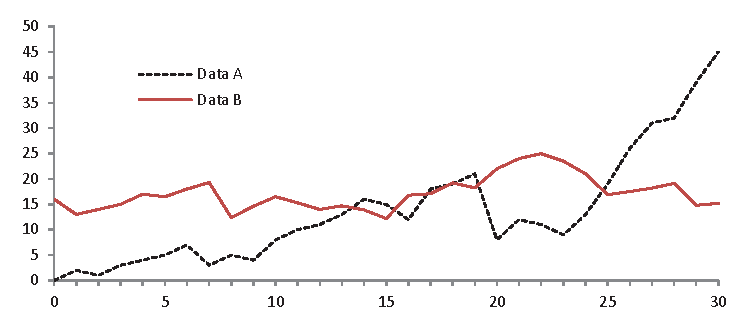
\includegraphics[width=0.6\textwidth]{fig1.eps}
		\centering
		\caption{A figure caption is always placed below the illustration.
			Please note that short captions are centered, while long ones are
			justified by the macro package automatically.} \label{fig1}
	\end{figure}
	
	\begin{theorem}
		This is a sample theorem. The run-in heading is set in bold, while
		the following text appears in italics. Definitions, lemmas,
		propositions, and corollaries are styled the same way.
	\end{theorem}
	%
	% the environments 'definition', 'lemma', 'proposition', 'corollary',
	% 'remark', and 'example' are defined in the LLNCS documentclass as well.
	%
	\begin{proof}
		Proofs, examples, and remarks have the initial word in italics,
		while the following text appears in normal font.
	\end{proof}
	For citations of references, we prefer the use of square brackets
	and consecutive numbers. Citations using labels or the author/year
	convention are also acceptable. The following bibliography provides
	a sample reference list with entries for journal
	articles~\cite{ref_article1}, an LNCS chapter~\cite{ref_lncs1}, a
	book~\cite{ref_book1}, proceedings without editors~\cite{ref_proc1},
	and a homepage~\cite{ref_url1}. Multiple citations are grouped
	\cite{ref_article1,ref_lncs1,ref_book1},
	\cite{ref_article1,ref_book1,ref_proc1,ref_url1}.
	
	
	\section*{Acknowledgements}
	
	Here is your acknowledgements. You may also include your feelings, suggestion, and comments in the acknowledgement section.
	
	%
	% ---- Bibliography ----
	%
	% BibTeX users should specify bibliography style 'splncs04'.
	% References will then be sorted and formatted in the correct style.
	%
	% \bibliographystyle{splncs04}
	% \bibliography{mybibliography}
	%
	\begin{thebibliography}{8}
		\bibitem{ref_article1}
		Author, F.: Article title. Journal \textbf{2}(5), 99--110 (2016)
		
		\bibitem{ref_lncs1}
		Author, F., Author, S.: Title of a proceedings paper. In: Editor,
		F., Editor, S. (eds.) CONFERENCE 2016, LNCS, vol. 9999, pp. 1--13.
		Springer, Heidelberg (2016).
		
		\bibitem{ref_book1}
		Author, F., Author, S., Author, T.: Book title. 2nd edn. Publisher,
		Location (1999)
		
		\bibitem{ref_proc1}
		Author, A.-B.: Contribution title. In: 9th International Proceedings
		on Proceedings, pp. 1--2. Publisher, Location (2010)
		
		\bibitem{ref_url1}
		LNCS Homepage, \url{http://www.springer.com/lncs}. Last accessed 4
		Oct 2017
	\end{thebibliography}
\end{document} 